\documentclass[UTF8]{ctexart}

\usepackage{CJK}
\usepackage{ctex}

\usepackage{geometry}% 版面大小
\geometry{a4paper,scale=0.7}

\usepackage{graphicx}
\graphicspath{{assets/}}
\usepackage{caption2}
\usepackage{subfigure}
\usepackage{float}

\usepackage[hidelinks]{hyperref}

\usepackage{listings} % packages for code blockings
\usepackage{xcolor}

\title{\textbf{作业2-2}}
\author{刘时宜 201180078}
\date{\today}

\begin{document}
    \maketitle
    \begin{figure}[H]
        \centering
        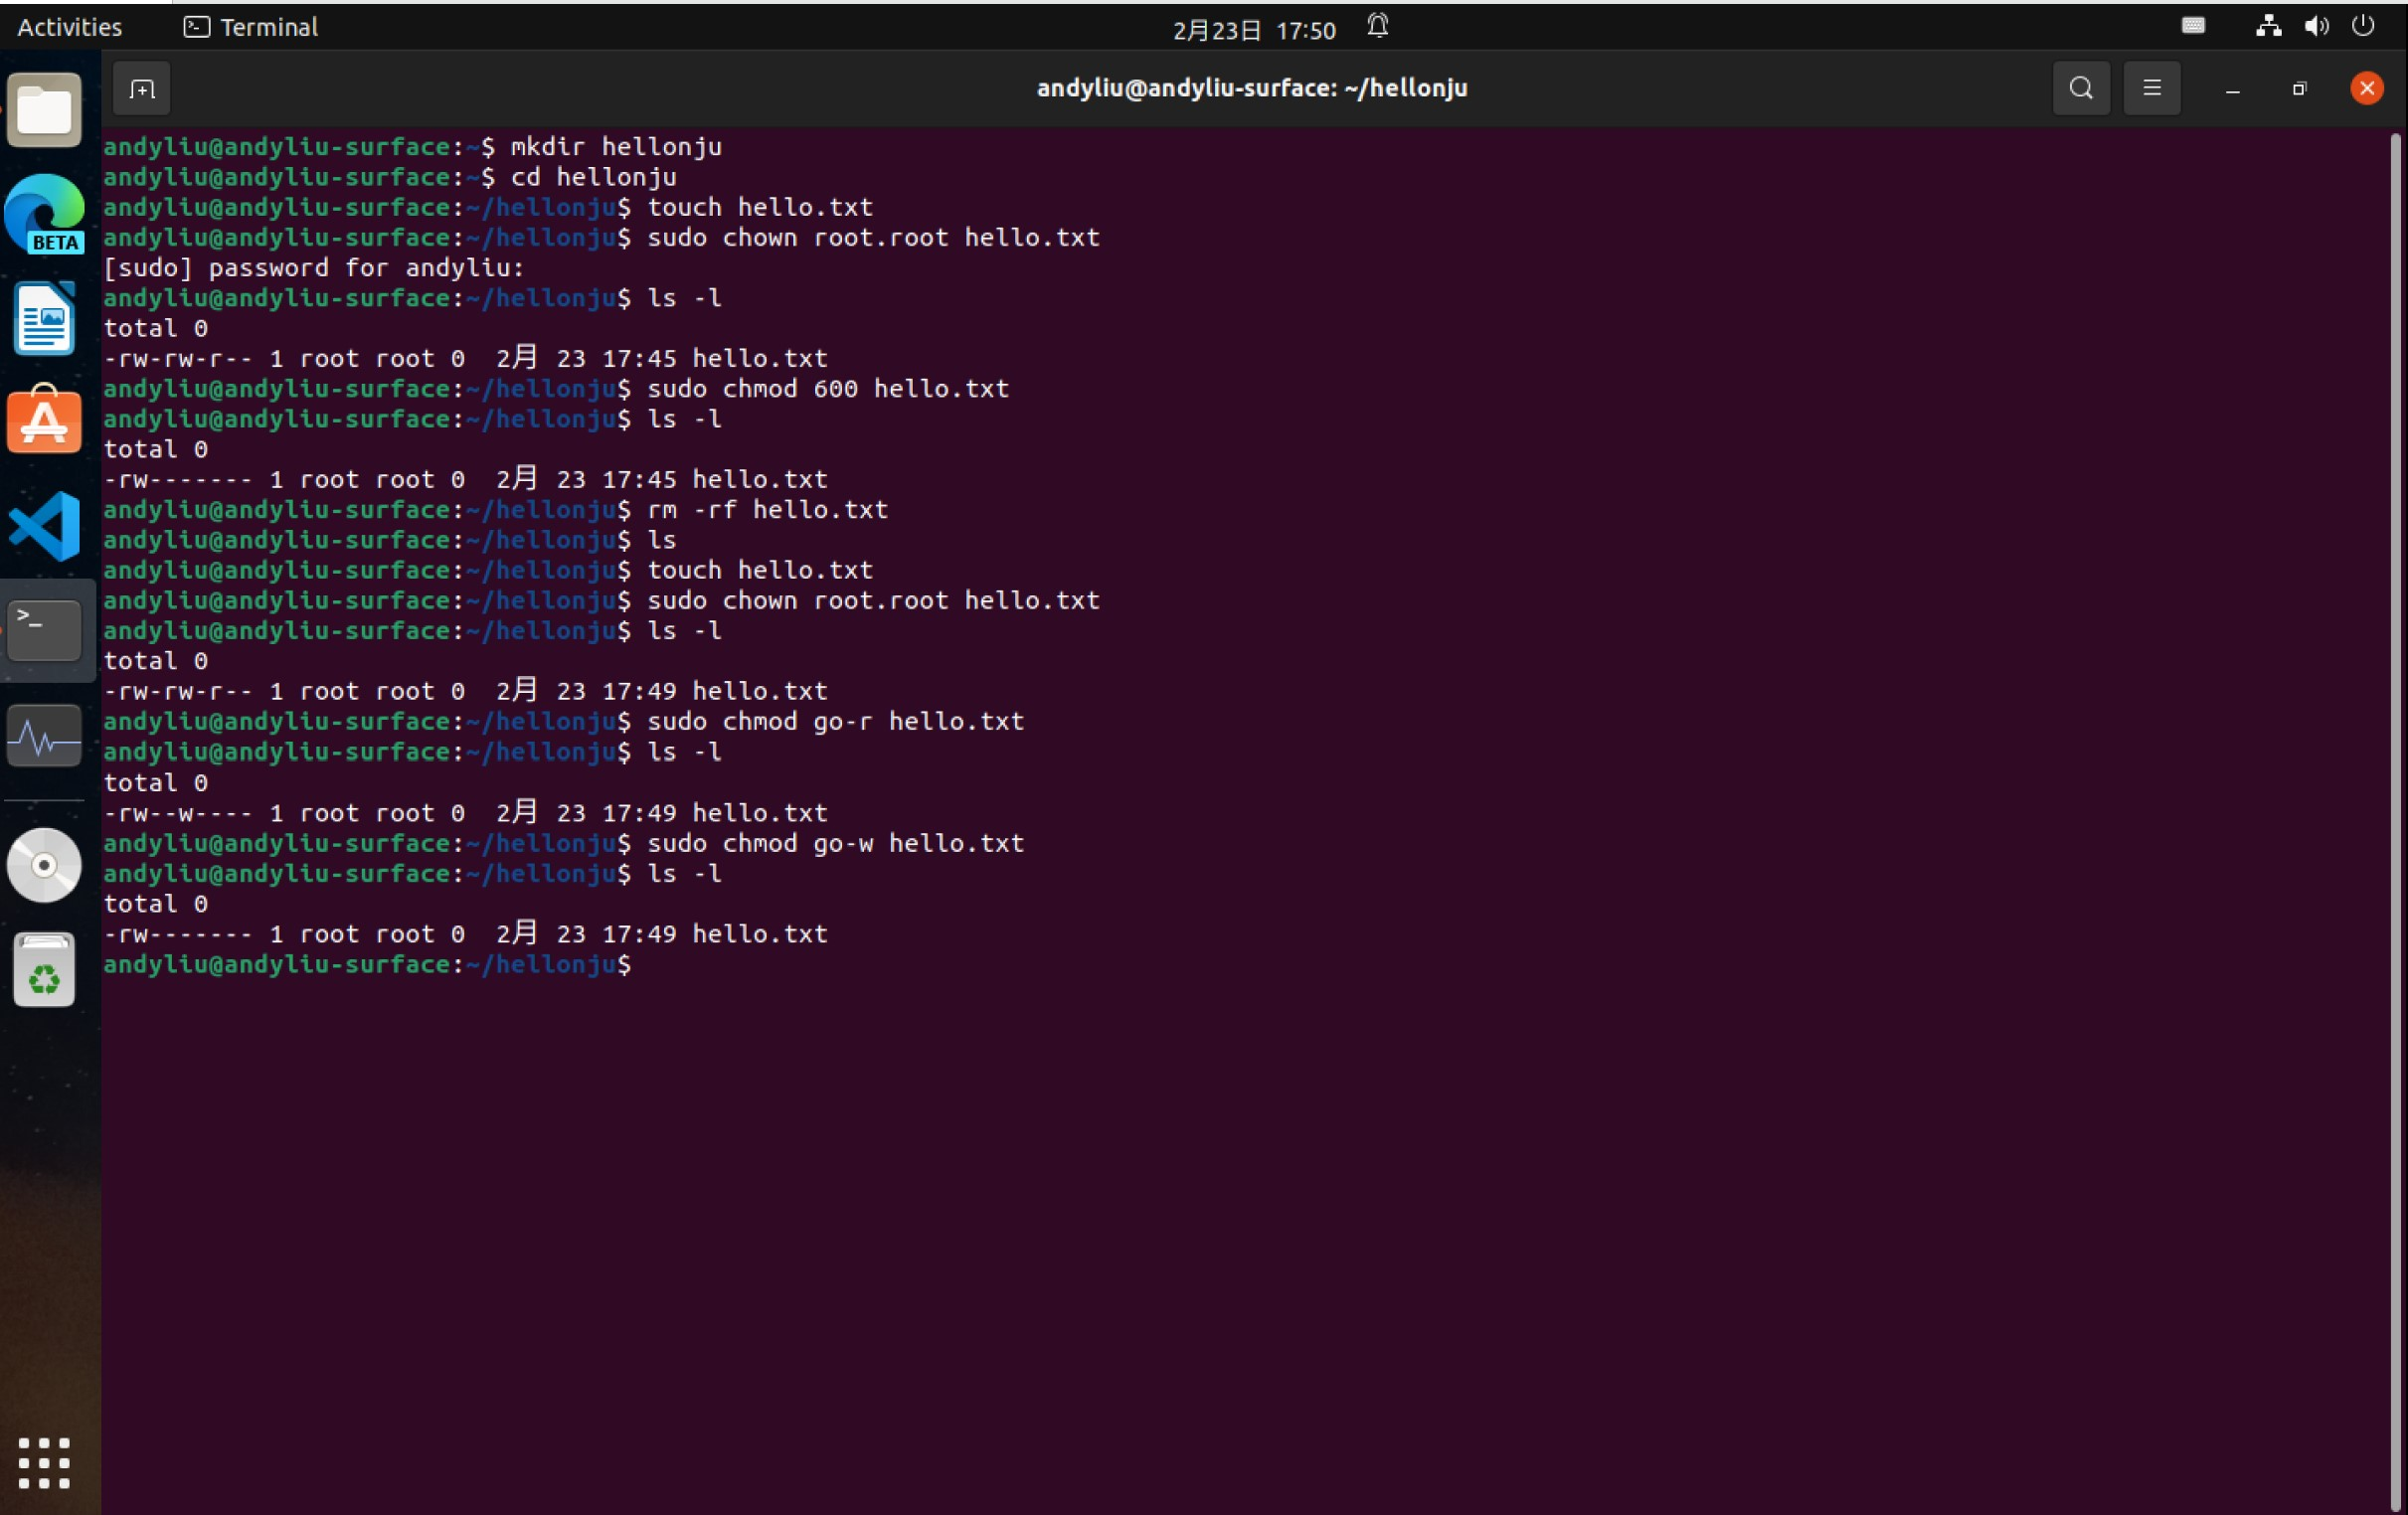
\includegraphics[width=0.8\textwidth]{hw2-2.jpg}
    \end{figure}
    逐条解释命令如下:
    \begin{enumerate}
        \item 在用户目录下创建目录hellonju
        \item 改变当前路径到hellonju
        \item 新建文件hello.text
        \item 改变属主为root.root
        \item 查看当前文件夹下文件的详细情况(含权限信息)
        \item 改变文件权限为600
        \item 查看当前文件夹下文件的详细情况(含权限信息),\textbf{已经成功完成任务}
        \item 删除文件(为了使用另一种方法改变文件权限)
        \item 查看当前文件夹下文件,确认删除成功
        \item 新建文件hello.text
        \item 改变属主为root.root
        \item 查看当前文件夹下文件的详细情况(含权限信息)
        \item 更改文件权限:减去组内用户和其他用户的读取权限
        \item 查看当前文件夹下文件的详细情况(含权限信息),确认权限更改情况
        \item 更改文件权限:减去组内用户和其他用户的写入权限
        \item 查看当前文件夹下文件的详细情况(含权限信息),确认权限更改情况,\textbf{已经成功完成任务}
    \end{enumerate}
\end{document}